\chapter{Literature Review}

Although the difficulty of strongly protecting confidential
information has been known for some time, the research
addressing this problem has had relatively little impact on the
design of commercially available computing systems. These
systems employ security mechanisms such as access control,
capabilities, firewalls and antivirus software; it is useful to see
how the these standard security mechanisms fall short. Access control is an important part of the current
security infrastructure. For example, a file may be assigned
access-control permissions that prevent users other than its
owner from reading the file; more precisely, these permissions
prevent processes not authorized by the file owner from
reading the file. However, access control does not control how
the data is used after it is read from the file. To soundly enforce
confidentiality using this access-control policy, it is necessary
to grant the file access privilege only to processes that will
not improperly transmit or leak the confidential data. But
these are precisely the processes that obey a much stronger
information-flow policy. Access-control mechanisms cannot
identify these processes; therefore, access control, while useful,
cannot substitute for information-flow control. 

Other common security enforcement mechanisms such as
firewalls, encryption and antivirus software are useful for protecting
confidential information. However, these mechanisms
do not provide end-to-end security. For example, a firewall
protects confidential information by preventing communication
with the outside. In practical systems, however, firewalls
permit some communication in both directions \cite{ref_64_box2000simple};
whether this communication violates confidentiality lies outside
the scope of the firewall mechanism. Similarly, encryption
can be used to secure an information channel so that only
the communicating endpoints have access to the information.
However, this encryption provides no assurance that once the
data is decrypted, the computation at the receiver respects the
confidentiality of the transmitted data. Antivirus software is
based on detecting patterns of previously known malicious
behavior in code and, thus, offers limited protection against
new attacks.

However, many intuitively secure programs do allow some release, or declassification, of secret information (such as- password checking, information purchase, and spreadsheet computation). Noninterference fails to recognize such programs as secure. In this respect, many security type systems enforcing noninterference are impractical. On the other side of the spectrum are type systems designed to accommodate some information leakage. However, there is often little or no guarantee about what is actually being leaked. As a consequence, such type systems are vulnerable to laundering attacks, which exploit declassification mechanisms to reveal more secret data than intended. To bridge this gap, Sabelfeld and Myers
\cite{ref_72_sabelfeld2004model} introduces a new security property, delimited release, an end-to-end guarantee that declassification cannot be exploited to construct laundering attacks. In addition, a security type system is given that straightforwardly and provably enforces delimited release.

If a user wishes to keep some data confidential, he or
she might state a policy stipulating that no data visible
to other users is affected by confidential data. This policy
allows programs to manipulate and modify private data, so
long as visible outputs of those programs do not improperly
reveal information about the data. A policy of this sort is a
noninterference policy \cite{ref_65_goguen1982security}, because it states that confidential
data may not interfere with (affect) public data. An attacker (or unauthorized user) is assumed to be allowed
to view information that is not confidential (that is public).
The usual method for showing that noninterference holds is
to demonstrate that the attacker cannot observe any difference
between two executions that differ only in their confidential
input \cite{ref_66_goguen1984unwinding}. Noninterference can be naturally expressed by
semantic models of program execution. This idea goes back
to Cohen's early work on strong dependency \cite{ref_67_cohen1977information}, \cite{ref_68_cohen1978information}.
McLean \cite{ref_69_mclean1992proving} argues for noninterference for programs in the
context of trace semantics. However, neither work suggests an
automatic security enforcement mechanism.

The type-checking approach has been implemented
in the Jif compiler \cite{ref_48_chong:jif,ref_40_myers:jflow}.
In the type-checking approach, every program expression
has a security type with two parts: an ordinary type such as int,
and a label that describes how the value may be used. Unlike
the labels used by mandatory access-control mechanisms,
these labels are completely static: they are not computed at
run time. Because of the way that type checking is carried
out, a label defines an information-flow policy on the use of
the labeled data. Security is enforced by type checking; the
compiler reads a program containing labeled types and in type checking
the program, ensures that the program cannot contain
improper information flows at run time. The type system
in such a language is a security-type system that enforces
information-flow policies.

This chapter described the basic of sanitization, declassification and authentication mechanism in software and web application. Also here the purpose and requirements of those three functions (sanitization, declassification and authentication) are presented. At last of this chapter the mechanism of detecting information flow errors during design and code also presented.

\section{Sanitization}
Sanitization is the process of removing sensitive information from a document or other message or sometimes encrypting messages, so that the document may be distributed to a broader audience. Sometimes sanitization can be called as an operation that ensures that user input can be safely used in an SQL query. Web applications use malicious input as part of a sensitive operation without having properly checked or sanitized the input values from the user. Previous research on vulneribility analysis has mostly focused on identifying cases which web applications directly uses external input for critical operations. It is suggested that always use proper sanitization method to validate external input values from the user for any application.For example, user inputs must always flow through a sanitizing function before flowing into a SQL query or HTML, to avoid SQL injection or cross-site scripting vulnerabilities.

Reflection of security breaches are very significant for high assurance system. For examples of this type of systems are aircraft navigation, where a fault could lead to a crash, various control systems which has critical infrastructure , where an error 
could cause toxic waste to leak, and weapons targeting, where an inaccuracy could result in severe collateral damage. In such
operational environments, the impact is virtually irreversible and must therefore be prevented even if it is likely to occur
with low probability.It's always good that transforming information to a form which is suitable for release or sanitize the information by redacting some portions of it.

Three of the top five most common website attacks are SQL injection, cross-site scripting (XSS), and remote file inclusion (RFI). The root cause of these attacks is common: input sanitization. All three exploits are leveraged by data sent to the web server by the end user. When the end user is a good guy, the data he sends the server is relevant to his interaction with the website. But when the end user is a hacker, he/she can exploit this mechanism to send the web server input which is deliberately constructed to escape the legitimate context and execute unauthorized actions.

SQL injection vulnerabilities arise in applications where elements of a SQL query originate from an untrusted source. Without precautions, the untrusted data may maliciously alter the query, resulting in information leaks or data modification. The primary means of preventing SQL injection are sanitization and validation, which are typically implemented as parameterized queries and stored procedures.

Suppose a system authenticates users by issuing the following query to a SQL database. If the query returns any results, authentication succeeds; otherwise, authentication fails.

\begin{lstlisting}
	SELECT * FROM db_user WHERE username='<USERNAME>' AND
	password='<PASSWORD>'
\end{lstlisting}

Suppose an attacker can substitute arbitrary strings for <USERNAME> and <PASSWORD>. In that case, the authentication mechanism can be bypassed by supplying the following <USERNAME> with an arbitrary password:

\begin{lstlisting}
	validuser' OR '1'='1
\end{lstlisting}

The authentication routine dynamically constructs the following query:

\begin{lstlisting}
	SELECT * FROM db_user WHERE username='validuser' OR '1'='1' AND password='<PASSWORD>'
\end{lstlisting}

If validuser is a valid user name, this SELECT statement yields the validuser record in the table. The password is never checked because username='validuser' is true; consequently, the items after the OR are not tested. As long as the components after the OR generate a syntactically correct SQL expression, the attacker is granted the access of validuser.
Similarly, an attacker could supply the following string for PASSWORD with an arbitrary username:

\begin{lstlisting}
	' OR '1'='1
\end{lstlisting}
producing the following query:

\begin{lstlisting}
	SELECT * FROM db_user WHERE username='<USERNAME>' AND password='' OR '1'='1'
\end{lstlisting}
'1'='1' always evaluates to true, causing the query to yield every row in the database. In this scenario, the attacker would be authenticated without needing a valid username or password.


In many cases, the data is passed directly to a component in a different trusted domain. Data sanitization is the process of ensuring that data conforms to the requirements of the subsystem to which it is passed. Sanitization also involves ensuring that data conforms to security-related requirements regarding leaking or exposure of sensitive data when output across a trust boundary. Sanitization may include the elimination of unwanted characters from the input by means of removing, replacing, encoding, or escaping the characters. Sanitization may occur following input (input sanitization) or before the data is passed across a trust boundary (output sanitization). Data sanitization and input validation may coexist and complement each other. Many command interpreters and parsers provide their own sanitization and validation methods. When available, their use is preferred over custom sanitization techniques because custom-developed sanitization can often neglect special cases or hidden complexities in the parser. Another problem with custom sanitization code is that it may not be adequately maintained when new capabilities are added to the command interpreter or parser software.

Input sanitization describes cleansing and scrubbing user input to prevent it from jumping the fence and exploiting security holes. But thorough input sanitization is hard. While some vulnerable sites simply don't sanitize at all, others do so incompletely, lending their owners a false sense of security.

Some basic purpose of sanitization are given below:
\begin{itemize}
	\item Remove malicious elements from the input.
	\item To identify the set of parameters and global variables which must be sanitized before calling functions.
	\item It is acceptable to first pass the untrusted user input through a trusted sanitization function.	
	\item Any user input data must flow through a sanitization function before it flows into a SQL query.
	\item Confidential data needs to be cleansed to avoid information leaks.
	\item Most paths that go from a source to a sink pass through a sanitizer.
	\item Developers typically define a small number of sanitization functions in libraries.
	\item Prevent web attacks using input sanitization.
\end{itemize}

\textbf{Sanitize the input by removing suspicious tags:}
This is a naive approach because it's almost impossible to cover everything. This regex function removes the obvious code to inject unwanted scripting which is given below.

\begin{lstlisting}
	public static String sanitize(String string) {
	return string
		.replaceAll("(?i)<script.*?>.*?</script.*?>", "")   // case 1
		.replaceAll("(?i)<.*?javascript:.*?>.*?</.*?>", "") // case 2
		.replaceAll("(?i)<.*?\\s+on.*?>.*?</.*?>", "");     // case 3
	}
	
\end{lstlisting}

\begin{itemize}
	\item case 1 : script tags are removed are removed.
	\item case 2 : javascript call are removed.
	\item case 3 : remove on* attributes like onLoad or onClick
\end{itemize}

\section{Declassification}
Information security has a challenge to address: enabling information flow controls with expressive information release (or declassification) policies. In a scenario of systems that operate on data with different sensitivity levels, the goal is to provide security assurance via restricting the information flow within the system. Practical security-typed languages support some form of declassification through which high-security information is allowed to flow to a low-security system or observer.

United States Federal Trade Commission reveals the damage that is continually caused by electronic information leakage. In protecting sensitive information, including everything from credit card information to military secrets to personal, medical information, there is a highly
need for software applications with strong, confidentiality guarantees.
Security-typed languages promise to be a valuable tool in making provably secure software applications. In such languages, each
data item is labeled with its security policy. In practical security-typed languages support some form of declassification, in which high-security information is permitted to flow to a low-security receiver/observer.

To declassify information means lowering the security classification of selected information. Sabelfeld and Sands \cite{ref_3_sabelfeld2009declassification} identify four different dimensions of declassification, what is declassified, who is able to declassify, where the declassification occurs and when the declassification takes place.

Myers and Liskov introduced the decentralized label model \cite{ref_4_myers2000protecting}, describing how labels could be applied
to a programming language and then used to check information
flow policy compliance in distributed systems. The framework
includes a declassify function for downgrading data if the
owners policies allow. The model allows principals to define their own downgrading policies.

\textbf{Dimensions of declassification:}
Classification of the basic declassification goals according to four axes: what information is released, who releases information, where in the system information is released and when information can be released.

\begin{itemize}
   \item What: Selective or Partial information flow policies \cite{ref_5_cohen1977information,ref_6_cohen1978information,ref_7_joshi2000semantic,ref_8_giacobazzi2005adjoining} regulate what
   information may be released. Partial release guarantees that only a part of a secret is
   released to a public domain. Partial release can be specified in terms of precisely which
   parts of the secret are released. This is useful,
   for example, when partial information about a credit card number or a social security number is used for logging.
   
   \item Who: In a computing system it is essential to specify who controls information release .
   Ignoring the issue of control opens up attacks where the attacker hijacks release
   mechanisms to launder secret information. Myers and Liskov decentralised label
   model \cite{ref_9_myers1997decentralized} security labels with explicit ownership information. According to this approach, information release of some data is safe if it is performed by the
   owner who is explicitly recorded in the data security label. This model has been used for enhancing Java with information flow controls \cite{ref_10_myers1999jflow} and has been implemented in
   the Jif compiler \cite{ref_11_myers2001jif}.
   
   \item Where: In a system information  Where is an important aspect of information release.One can ensure that no other  part can release further information.
   by delegating particular parts of the system to release information.Declassification
   via encryption is not harmful as long as the program is, in some sense, noninterfering
   before and after encryption.  A combination of \enquote{where} and \enquote{who} policies in the presence of encryption has
   been recently investigated by Hicks et al. \cite{ref_12_hicks2005declassification}
   
   \item When: The fourth dimension of declassification is  \enquote{when} information should be released.The work of Giambiagi and Dam \cite{ref_19_giambiagi2003secure} focuses on the correct implementation of security protocols. Here the goal is not to prove a noninterference property of the protocol, but to use the components of the protocol description as a specification of what and when information may be released.Chong and Myers security policies \cite{ref_13_chong2004security} address when information is released.By annotating variables this is achieved.
   
\end{itemize}

For a given model, the \enquote{what} and \enquote{when} dimensions seem relatively straightforward to define formally. The \enquote{what} dimension abstracts the extensional semantics
of the system; the \enquote{when} dimension can be distinguished from this since it requires an intensional semantics that (also) models time, either abstractly in terms of complexity
or via intermediate events in a computation. The \enquote{who} and \enquote{where} dimensions are
harder to formalize in a general way, beyond saying that they cannot be captured by the
\enquote{what} and \enquote{when} dimensions.

\section{Authentication}
Malicious applications targeting financial account information have increased dramatically over the last years. The number of online applications is growing strong. The ease of use of the Internet and the growing user base make a perfect target for criminals. Attacking thousands of users is achievable with only one click.The methods used by these criminals vary immensely, but they have one thing in common: they are getting more and more sophisticated. With these increasing threats, governments are issuing stronger legislations and companies are realizing that their current systems can not thwart current attacks anymore.

To counter these threats, current authentication systems have to be adopted. Not only the criminal side has made advances in the last years. The security industry developed new mechanisms and protection systems to thwart even the most sophisticated attacks.

Before describing the process of the authentication, need to explain some terms. Now-a-days, AAA is often used. AAA stands for Authentication, Authorization and Accounting. It is important to know the differences between those terms:
 
\textbf{Authentication}: the confirmation that a user is who it is claiming to be. 

\textbf{Authorization}: the process to determine whether the user has the authority to issue certain commands.
 
\textbf{Accounting}: measuring the resources a user consumes during access.


Authentication is the mechanism which confirms the identity of users trying to access a system. For a user to be granted access to a resource, they must first prove that they are who they claim to be. Generally this is handled by passing a key with each request (often called an access token, User verification using user id and password). The system or server verifies that the access token or user id and password is genuine, that the user does indeed have the required privileges to access the requested resource and only then the request granted.

Now-a-days following authentication, a user must gain authorization for doing certain tasks. After logging into a system, for instance, the user may try to issue commands. The authorization process determines whether the user has the authority to issue such commands. Simply put, authorization is the process of enforcing policies: determining what types or qualities of activities, resources, or services a user is permitted. Usually, authorization occurs within the context of authentication. Once you have authenticated a user, they may be authorized for different types of access or activity.

According to J Viega and G McGraw \cite{ref_92_viega2001building} the processes how to avoid the top ten software security flaws are:
\begin{itemize}
	\item Earn or give, but never assume, trust.
	
	\item Use an authentication mechanism that
	cannot be bypassed or tampered with.
	
	\item Authorize after you authenticate.
	
	\item Strictly separate data and control
	instructions, and never process control
	instructions received from untrusted sources.
	
	\item Define an approach that ensures all data are
	explicitly validated.

	\item Use cryptography correctly.
	 
	\item Identify sensitive data and how they should
	be handled.
	
	\item Always consider the users.

	\item Understand how integrating external
	components changes your attack surface.
	
	\item Be flexible when considering future changes
	to objects and actors.
	
	
\end{itemize}

Protecting confidential data in computing environments has long been recognized as a difficult and daunting problem. All modern operating systems include some form of access control to protect files from being read or modified by unauthorized users. However, access controls are insufficient to regulate the propagation of information after it has been released for processing by a program. Similarly,
cryptography provides strong confidentiality guarantees in open, possibly hostile environments like the Internet, but it is prohibitively expensive to perform nontrivial computations with encrypted data. Neither access control nor encryption
provide complete solutions for protecting confidentiality.

A complementary approach, proposed more than thirty years ago, is to track and regulate the information flows of the system to prevent secret data from leaking to unauthorized parties. This can be done either dynamically, by marking data with a label describing its security level and then propagating those labels to all derivatives of the data, or statically, by analyzing the software that processes
the data to determine whether it obeys some predefined policy with respect to the data. Arguably, a mostly static approach (perhaps augmented with some dynamic checks) is the most promising way of enforcing information-flow policies.

Also authentication can be defined as it is the process by which the system validates a user's logon information. A user's name and password are compared to an authorized list and if the system detects a match then access is granted to the extent specified in the permission list for that user.

One familiar use of authentication and authorization is access control. A computer system that is supposed to be used only by those authorized must attempt to detect and exclude the unauthorized. Common examples of access control involving authentication include:
\begin{itemize}	
	\item A computer program using a blind credential to authenticate to another program.
	\item Logging in to a computer.	
	\item Using an Internet banking system.
	\item Withdrawing cash from an ATM and more
	\item Assurance of identity of person or originator of data.
\end{itemize}

 A variety of authentication technologies have hit the market over the years.To better understand what they are and how they compare to the user name/password combination, it helps to be familiar with the standard authentication factors something you know, something you have and something you are and how each technology leverages them to power its authentication capabilities.
 \begin{itemize}	
	\item Something you know is a bit of knowledge committed to memory, such as a password or
	 an answer to a secret question.
	\item Something you have is an item that is owned or carried, such as a smart card or similar
	 hardware device.
	\item	 Something you are is a physical attribute that can be identified, such as a fingerprint or voice.
\end{itemize}

\textbf{The Challenges in secure Authentication:}

The security of an application is always a trade off between a high level of security and more usability. The more security is added to an authentication system (pass phrases instead of passwords, multiple authentication tokens), the lower will be the acceptance rate of the users and the usability will decrease. It is a big challenge to find the most secure authentication system which is accepted by the users. 

Users always want new applications and features with easy to use interfaces. At the same time they are worried about the increasing dangers. Moreover, new legislations are pushing manufactures and companies to protect the privacy of their clients.The increasing mobility of the users is another important factor. The users want to access their applications not only with their desktop at home, but also in their office, on vacation with their PDA and everywhere with their cell phone. Those needs pose significant requirements to the security of applications. 

These broad demands from the users create a wide range of attack vectors. Phishing, identity theft, spyware, malware, keyloggers, javascript attacks, and generally untrusted consumer platforms all make the traditional means of password based authentication ever more complicated.


According to the networkworld \cite{ref_21_networld} now-a-days seven strong authentication methods are:
\begin{itemize}
\item Computer recognition software.
\item Biometrics
\item E-mail or SMS one-time password (OTP).
\item One Time Password (OTP) token.
\item Out of band.
\item Peripheral device recognition.
\item Scratch-off card.
\end{itemize}	

\section{Static Code Analysis}

Static program analysis is the analysis of computer software that is performed without actually executing programs (analysis performed on executing programs is known as dynamic analysis). In most cases the analysis is performed on some version of the source code, and in the other cases, some form of the object code.The term is usually applied to the analysis performed by an automated tool, with human analysis being called program understanding, program comprehension, or code review. Software inspections and Software walkthroughs are also used in the latter case. .Static analysis, also called static code analysis, is a method of computer program debugging that is done by examining the code without executing the program. The process provides an understanding of the code structure, and can help to ensure that the code adheres to industry standards. Automated tools can assist programmers and developers in carrying out static analysis. The process of scrutinizing code by visual inspection alone (by looking at a printout, for example), without the assistance of automated tools, is sometimes called program understanding or program comprehension \cite{ref_86_techtarget:techtarget}.

The principal advantage of static analysis is the fact that it can reveal errors that do not manifest themselves until a disaster occurs weeks, months or years after release. Nevertheless, static analysis is only a first step in a comprehensive software quality-control regime. After static analysis has been done, dynamic analysis is often performed in an effort to uncover subtle defects or vulnerabilities. In computer terminology, static means fixed, while dynamic means capable of action and/or change. Dynamic analysis involves the testing and evaluation of a program based on execution. Static and dynamic analysis, considered together, are sometimes referred to as glass-box testing \cite{ref_86_techtarget:techtarget}.

Static code analysis advantages are:
\begin{itemize}
	\item It can find weaknesses in the code at the exact location.
	\item It can be conducted by trained software assurance developers who fully understand the code.
	\item It allows a quicker turn around for fixes.
	\item It is relatively fast if automated tools are used.
	\item Automated tools can scan the entire code base.
	\item Automated tools can provide mitigation recommendations, reducing the research time.
	\item It permits weaknesses to be found earlier in the development life cycle, reducing the cost to fix.
\end{itemize}

According to the GCN \cite{ref_87_gcn:gcn} static code analysis limitations are:
\begin{itemize}
	\item It is time consuming if conducted manually.
	\item Automated tools do not support all programming languages.
	\item Automated tools produce false positives and false negatives.
	\item There are not enough trained personnel to thoroughly conduct static code analysis.
	\item Automated tools can provide a false sense of security that everything is being addressed.
	\item Automated tools only as good as the rules they are using to scan with.
	\item It does not find vulnerabilities introduced in the runtime environment.
\end{itemize}

\section{Information Flow Vulnerabilities}

Information flow means  transmission of information from one "place" to another. Securing the data manipulated by computing systems has been a challenge in the past years. Several methods to limit the information disclosure exist today, such as access control lists, firewalls, and cryptography. However, although these methods do impose limits on the information that is released by a system, they provide no guarantees about information propagation. For example, access control lists of file systems prevent unauthorized file access, but they do not control how the data is used afterwards. Similarly, cryptography provides a means to exchange information privately across a non-secure channel, but no guarantees about the confidentiality of the data are given once it is decrypted.

In low level information flow analysis, each variable is usually assigned a security level. The basic model comprises two distinct levels: low and high, meaning, respectively, publicly observable information, and secret information. To ensure confidentiality, flowing information from high to low variables should not be allowed. On the other hand, to ensure integrity, flows to high variables should be restricted.For example, considering two security levels L and H (low and high), if L less equal to H, flows from L to L, from H to H, and L to H would be allowed, while flows from H to L would not \cite{ref_88_smith2007principles}.

A system is secure with respect to confidentiality
should arise from a rigorous analysis showing that the system
as a whole enforces the confidentiality policies of its users.
This analysis must show that information controlled by a confidentiality policy cannot flow to a location where that policy
is violated. The confidentiality policies we wish to enforce
are, thus, information-flow policies and the mechanisms that
enforce them are information-flow controls. Information-flow
policies are a natural way to apply the well-known systems
principle of end-to-end design \cite{ref_89_saltzer1984end} to the specification of
computer security requirements; therefore, we also consider
them to be specifications of end-to-end security. In a truly
secure system, these confidentiality policies could be precisely
expressed and translated into mechanisms that enforce them.
However, practical methods for controlling information flow
have eluded researchers for some time.

Information flow can be classified as explicit (information flow
that arises explicitly, due to assignment statements), and implicit
(flow that arises implicitly, due to conditional statements). In \cite{ref_90_liu2008static}, proposed a new general-purpose static analysis for the inference
of explicit information flow. This analysis is light-weight,works directly on Java programs before program execution, and
does not require annotations by the programmer. It can be incorporated
in program understanding and verification tools and help
verify in a practical manner the confidentiality and integrity of sensitive program data. We believe that our work, although limited in
the sense that it does not handle implicit flow, is a step forward towards
the use of static analysis for the purposes of reasoning about
information flow; it may help advance the use of static analysis in
tools for understanding and verification of security properties.


\section{ Detecting Information Flow Errors During Design}
If a step of function call like authentication, sanitization or declassification is missing inside the program then this can lead to software vulnerabilities. In the figure \ref{figure_FunctionCallMissing} left side picture depicted that it has three functions. Among them func2() is named either sanitization/declassification/authentication function. Which means in this scenario there will be no error regarding sanitization/declassification/authentication function. On the other hand the right side picture represents there is a missing function of sanitization/declassification/authentication function. That's why it is the buggy path of UML state charts during design stage of software life cycle. 
\begin{figure}[htbp]
	\centering
	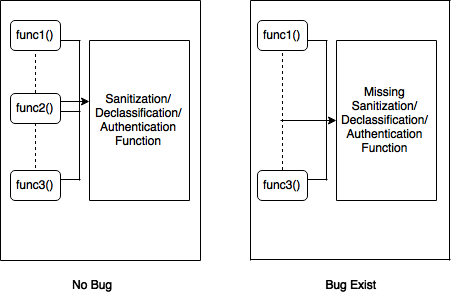
\includegraphics{styles/FunctionCallMissing.png}
	\caption{Information flow errors during design}
	\label{figure_FunctionCallMissing}
\end{figure}


\section{ Detecting Information Flow Errors During Coding}

Figure \ref{figure_bug_detection_during_coding} depicts two explicit information flows according to A lattice model of secure information flow of Denning \cite{ref_14_denning1976lattice} contained in two systems (system 1) and (system 2)
where each of the flows starts with statement variable a and ends with leaving the system. The the variable declaration up to outside the system represent C language statements. System 1 is depicted in left side containing the flow from the source to the sink and leaving the system indicated with circles at the top and bottom of each of the
two information flows. A source is any function or programming language statement which provides private information through a system boundary. A sink can be a function call or programming language statement which exposes private information to the outside of the system through a system boundary. A system boundary can be a statement, function call, class, package or module. In figure 2.2 the source and sink represent C language statements where information enters and respectively leaves system 1 or system 2. The variable a was tagged with label \enquote{H} (confidential) as it inserts confidential information into system 1. The arrows represent the passing of the confidential label \enquote{H} between the program statements. When a variable labeled with \enquote{H} is about to leave system 1 or system 2 without passing through either authentication/declassifiaction/sanitization function then a bug report should be created.In figure 2 right side system has a bug because it passes a secured/confidential information without passing through authentication/declassifiaction/sanitization function. These functions either authenticated,declassified or sanitized  secured/confidential information and makes the variable label as \enquote{L} to leave the system. But in the left part of the picture there is no bug as in this system, secured/confidential information and the variable which is labeled with \enquote{H} passes through either authentication/declassifiaction/sanitization function.

\begin{figure}[htbp]
	\centering
	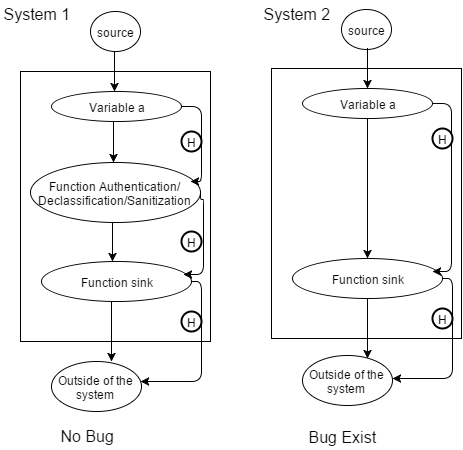
\includegraphics{styles/bug_detection_during_coding.png}
	\caption{Information flow errors during coding}
	\label{figure_bug_detection_during_coding}
\end{figure}
